% Tipo de documento
\documentclass[16pt,spanish]{article}

% Ruta a la plantilla
\def \plpath{.}

% Paquetes
% Importaciones y paquetes %%%%%%%%%%%%%%%%%%%%%%%%%%%%%%%%%%%%%%

% Codificación
\usepackage[utf8]{inputenc}
\usepackage[spanish,activeacute]{babel}

% Paquetes extras
\usepackage{listings} % Trozos de código
\usepackage{graphicx} % Imágenes
\usepackage{fancyhdr} % Cabeceras
\usepackage{lscape}   % Apaisado
%\usepackage{hyperref} % Enlaces
\usepackage{float} % para que H funcione en figure
%\usepackage[left=2.5cm,top=2.5cm,right=2cm,bottom=2.5cm]{geometry}

% Configuración  %%%%%%%%%%%%%%%%%%%%%%%%%%%%%%%%%%%%%%%%%%%%%%%%%

\lstset{language=C++,
	showstringspaces=true}

% Figura centrada con \figura{proporcion}{ruta}{caption}{label}
% Ejemplo de uso: \figura{0.5}{img.png}{Boceto}{figura1}
% El argumento proporción es opcional y por defecto es el ancho del texto
%
%                 nargs   defaults
\newcommand{\figura}[4][1]{
\begin{figure}[H!] % Aparecerá justo donde está el código
	\centering
	     \includegraphics[width=#1\textwidth]{#2}
	\caption{#3}
	\label{#4}
\end{figure}
}

% Figura centrada y rotada 90º a la derecha
% con \figura{proporcion}{ruta}{caption}{label}
% Ejemplo de uso: \figura{0.5}{img.png}{Boceto}{figura1}
% El argumento proporción es opcional y por defecto es el ancho del texto
%
%                 nargs   defaults
\newcommand{\figuraApaisada}[4][1]{
\begin{figure}[H!] % Aparecerá justo donde está el código
	\centering
	     \includegraphics[width=#1\textwidth,angle=90]{#2}
	\caption{#3}
	\label{#4}
\end{figure}
}




%  Datos del documento a Editar %%%%%%%%%%%%%%%%%%%%%%%%%%%%%%%%%%%

% Título del documento
\def \titlename{IberOgre y Sion Tower}
\def \subtitlename{Memoria para el V CUSL}

% Autores separados por \and
\def \authorname{David Saltares Márquez}

% Versión de la revisión (En blanco para documentos nuevos)
\def \revname{1} % Ponemos un espacio para evitar errores en la cabecera.

% Fecha (En blanco para la fecha de hoy)
\def \datename{}

% Variables a usar para mantener un sistema consistente
\def \proyecto{\emph {IberOgre y Sion Tower} }
\def \juego{\emph {Sion Tower} }
\def \wiki{\emph{IberOgre} }

% Configuración  %%%%%%%%%%%%%%%%%%%%%%%%%%%%%%%%%%%%%%%%%%%%%%%%%

\title{\titlename}
\author{\authorname}
%\date{\datename}

% Cabecera y pie del documento
\pagestyle{fancy}
%\renewcommand{\headrulewidth}{0.2pt}
%\fancyhead[HC]{ {\footnotesize \titlename} }
%\fancyhead[FR]{ {\footnotesize \thepage} }
%\fancyhead{}
%\fancyfoot{}


%%%%%%%%%%%%%%%%%%%%%%%%%%%%%%%%%%%%%%%%%%%%%%%%%%%%%%%%%%%%%%%%%

\begin{document}

% Portada %%%%%%%%%%%%%%%%%%%%%%%%%%%%%%%%%%%%%%%%%%%%%%%%%

% -*-portada.tex-*-
% Este fichero es parte de la plantilla LaTeX para
% la realización de Proyectos Final de Carrera, protejido
% bajo los términos de la licencia GFDL.
% Para más información, la licencia completa viene incluida en el
% fichero fdl-1.3.tex

% Fuente tomada del PFC 'libgann' de Javier Vázquez Púa

\begin{titlepage}

  \begin{center}

    
\includegraphics[scale=0.2]{logo_uca.png} \\
    
    \vspace{2.0cm}
    
    \LARGE{\textbf{ESCUELA SUPERIOR DE INGENIERÍA}} \\
    
    \vspace{1.0cm}
    
    \Large{\textbf{INGENIERÍA TÉCNICA EN INFORMÁTICA DE GESTIÓN}} \\
    
    \vspace{3.0cm}
    
    \Large{IBEROGRE, WIKI DE OGRE3D EN ESPAÑOL\\Y SION TOWER, VIDEOJUEGO DE ESTRATEGIA}\\
    
    \vspace{2.0cm}
    
    \Large{David Saltares Márquez} \\
  
    \vspace{0.5cm}

    \large{\today}
    
  \end{center}
\end{titlepage}


% Índice %%%%%%%%%%%%%%%%%%%%%%%%%%%%%%%%%%%%%%%%%%%%%%%%%%

\tableofcontents
\cleardoublepage

% Cambios en esta Revisión %%%%%%%%%%%%%%%%%%%%%%%%%%%%%%%%%%%%%%

%\section{Cambios}
%\label{sec:cambios} 


%\paragraph{}
%Cambios con respecto a versiones anteriores del documento.

%\begin{itemize}
%	\item {\bf Revision 1}
%		\begin{itemize}
%			\item Cambio1
%			\item Cambio2
%		\end{itemize}
%\end{itemize}

%%%%%%%%%%%%%%%%%%%%%%%%%%%%%%%%%%%%%%%%%%%%%%%%%%%%%%%%%%%%%%%%%

\section{Introducción}

\paragraph{}
En este texto se proporciona información a modo de resumen sobre los
objetivos, motivaciones, desarrollo y logros del proyecto \proyecto.
Para detalles adicionales es recomendable acudir a las fuentes que se
citan a lo largo del texto como el blog de desarrollo o la forja en Red Iris.

\paragraph{IberOgre}
es una wiki en español sobre desarrollo de videojuegos en 3D
utilizando el motor de renderizado Ogre. Surge principalmente ante la
inexistencia de documentación al respecto en castellano. No solo está
dirigida a cubrir el uso del mencionado motor sino que también trata
los conceptos matemáticos y físicos mínimos para desarrollar juegos
tridimensionales.

\paragraph{}
\wiki se aloja en los servidores de la Oficina de Software Libre de la
Universidad de Cádiz (OSLUCA):

\begin{verbatim}
    http://osl2.uca.es/iberogre
\end{verbatim}

\begin{figure}[H]
    \centering
        
\includegraphics[width=7cm]{img/iberogre.png} 
    \caption{Logo del proyecto \wiki}
    \label{img:logo-iberogre}
\end{figure}

\paragraph{Sion Tower}
es un videojuego de estrategia y acción multiplataforma (GNU/Linux y Windows)
con elementos de fantasía en 3D cuyo objetivo principal es servir
de ejemplo final a \wiki aunque tiene un claro componente lúdico para los
usuarios de escritorio. Controlamos a un joven mago que debe defender
la Torre Sagrada de una invasión mientras sus compañeros están celebrando
un rito. Cada nivel corresponde a un piso de la torre y el objetivo consiste
en evitar que los enemigos lleguen al centro del mismo empleando hechizos
y colocando trampas.

\paragraph{}
Está desarrollado en C++ utilizando bibliotecas libres como Ogre, OIS, SDL,
SDL mixer y pugixml. 

\begin{figure}[H]
    \centering
        
\includegraphics[width=9cm]{img/siontower.png} 
    \caption{Logo del proyecto \juego}
    \label{img:logo-siontower}
\end{figure}

\section{Motivaciones y objetivos}

\paragraph{}
En esta sección se exponen las motivaciones que me llevaron a embarcarme
en este proyecto así como los objetivos que me he propuesto cumplir de cara
al V Concurso Universitario de Software Libre y más allá.

\subsection{IberOgre}

\begin{itemize}
    \item Proporcionar documentación en castellano sobre desarrollo de
    videojuegos en 3D en un panorama de vacío al respecto.
    \item Especial atención y soporte a herramientas de desarrollo libres
    ya que la mayoría de documentación en inglés se centra en software privativo.
    \item Aunar los conceptos de geometría del espacio y uso de un motor 3D
    para que el lector no se vea obligado a acudir a decenas de fuentes
    diferentes.
    \item Ayudar al usuario a dar el salto de las 2D a las 3D. \wiki podría
    considerarse como una extensión de \emph{Wikijuegos}
    \footnote{Wikijuegos: http://osl.uca.es/wikijuegos}, una wiki
    sobre desarrollo de videojuegos en 2D utilizando libSDL alojada también
    en la OSLUCA.
    \item Ofrecer artículos con ejemplos y ejercicios prácticos para que el usuario
    comprenda el funcionamiento de Ogre y amplíe sus conocimientos por sí
    mismo.
    \item Seguir buenas prácticas para desarrollar software multiplataforma.
    \item Crear una comunidad que aprenda y colabore activamente en la creación
    de nuevo contenido.
\end{itemize}

\subsection{Sion Tower}

\begin{itemize}
    \item Deseo personal de aprender a desarrollar juegos en 3D.
    \item Proporcionar una aplicación lo más realista posible de los
    conocimientos expuestos en \wiki.
    \item Ofrecer información extensa sobre el proceso de desarrollo completo
    de un videojuego.
    \item Liberar los elementos del motor (debidamente documentados) más
    suceptibles a ser reutilizados en otros proyectos.
    \item Formar un pequeño equipo multidisciplinar que colabore aportando
    contenido multimedia al proyecto: arte 2D/3D, música y efectos de sonido.
    \item Motor extensible orientado a la creación de contenidos como
    niveles adicionales.
\end{itemize}

\section{Enlaces}

\paragraph{}
Se adjunta la lista de enlaces en los que encontrar información adicional
del proyecto \proyecto.

\begin{figure}[H]
    \centering
        
\includegraphics[width=9cm]{img/enlaces.png} 
    \caption{Medios con información sobre \proyecto}
    \label{img:enlaces}
\end{figure}

\begin{itemize}
    \item Blog de desarrollo: noticias, anuncios, experiencias, anécdotas y
    documentación sobre el proceso de desarrollo.
    \begin{verbatim}http://siondream.com/blog/category/proyectos/pfc\end{verbatim}
    \item Forja: repositorio Subversion, noticias, sistema de gestión de
    tareas y ficheros publicados.
    \begin{verbatim}https://forja.rediris.es/projects/cusl5-iberogre\end{verbatim}
    \item Web estática de la forja: información básica y enlaces a todos estos
    medios aprovechando el buen posicionamiento en buscadores de Red Iris.
    \begin{verbatim}http://cusl5-iberogre.forja.rediris.es\end{verbatim}
    \item Twitter: noticias, detalles del desarrollo y contacto cercano
    con los seguidores del proyecto.
    \begin{verbatim}http://twitter.com/iberogre\end{verbatim}
    \item Canal de Youtube: vídeos sobre las distintas fases del desarrollo
    de \juego.
    \begin{verbatim}http://youtube.com/user/davidsaltares\end{verbatim}
\end{itemize}

\section{Requisitos y dependencias}

\paragraph{}
Para poder compilar y ejecutar tanto los ejemplos de \wiki como las pruebas
(directorio branches) o versión estable (trunk) de \juego es necesario
instalar las versiones de desarrollo de Ogre y de las bibliotecas que se utilizan
de forma auxiliar como OIS, SDL y SDL mixer.

\paragraph{}
Es posible encontrar detalles adicionales en los artículos correspondientes
de \wiki:

\begin{itemize}
    \item Instalación de Ogre3D 1.7 en GNU/Linux
    \item Instalación de Ogre3D 1.7 en Windows
\end{itemize}

\begin{figure}[H]
    \centering
        
\includegraphics[width=5cm]{img/linux-windows.png} 
    \caption{Todo el código de \proyecto es multiplataforma}
    \label{img:linux-windows}
\end{figure}

\subsection{Instalación en GNU/Linux}

\paragraph{}
La instalación de los paquetes supone una distribución basada en Debian
como Ubuntu, en caso de utilizar otra distribución el proceso no debe
diferir en exceso del que se expone a continuación.

\begin{enumerate}
    \item Instalar las dependencias de Ogre:    
    \begin{verbatim}
sudo apt-get install g++ make libfreetype6-dev libboost-date-time-dev \
  libboost-thread-dev nvidia-cg-toolkit libfreeimage-dev zlib1g-dev \
  libzzip-dev libois-dev libcppunit-dev doxygen libxt-dev libxaw7-dev \ 
  libxxf86vm-dev libxrandr-dev libglu-dev cmake
    \end{verbatim}
    \item Descargar el código fuente de la última versión de Ogre desde
    la web oficial:
    \begin{verbatim}
http://www.ogre3d.org/download/source
    \end{verbatim}
    \item Descomprimimos el paquete y accedemos desde la terminal.
    \item Creamos un makefile dependiente de nuestra plataforma con cmake,
    compilamos e instalamos con make:
    \begin{verbatim}
cmake .
make
sudo make install
    \end{verbatim}
    \item Copiamos las bibliotecas de Ogre para no tener que distribuirlas
    con cada prueba:
    \begin{verbatim}
sudo cp lib/* /usr/lib/
    \end{verbatim}    
    \item Instalamos OIS (Object Oriented Input System), SDL y SDL mixer:
    \begin{verbatim}
sudo apt-get install libois-dev libsdl1.2-dev libsdl-mixer1.2-dev
    \end{verbatim} 
\end{enumerate}

\subsection{Instalación en Windows}

\begin{enumerate}
    \item Descargar una versión de MinGW que contenga GCC 4.5 o superior.
    \item Instalar el paquete en \emph{C:/mingw} y añadir \emph{C:/mingw/bin}
    a la variable de entorno \emph{PATH}.
    \item Instalar el editor de flujo sed, utilizado para generar las dependencias
    en los makefiles. Añadir su ruta a la variable de entorno \emph{PATH}.
    \begin{verbatim}
http://downloads.sourceforge.net/gnuwin32/sed-4.2-1-setup.exe
    \end{verbatim}
    \item Descargar e instalar la versión para MinGW de Ogre desde la web oficial:
    \begin{verbatim}
http://www.ogre3d.org/download/sdk
    \end{verbatim}
    \item Establecer la variable de entorno \emph{OGRE\_HOME} que apunte
    al directorio de intalación de Ogre.
    \item Establecer la variable de entorno \emph{BOOST\_ROOT} que apunte
    al directorio boost dentro de la instalación de Ogre.
    \item Descargar e instalar SDL y SDL mixer para MinGW.
\end{enumerate}

\subsection{Compilación en GNU/Linux}

\paragraph{}
Para compilar cualquier ejemplo de \wiki o el juego \juego en GNU/Linux 
es necesario acceder al directorio desde una terminal y ejecutar:

\begin{verbatim}
    # Modo debug
    make
    
    # Modo release
    make modo=release
\end{verbatim}

\subsection{Compilación en Windows}

\paragraph{}
Para compilar cualquier ejemplo de \wiki o el juego \juego en Windows 
es necesario acceder al directorio desde una terminal y ejecutar:

\begin{verbatim}
    # Modo debug
    make -f makefile-windows
    
    # Modo release
    make -f makefile-windows modo=release
\end{verbatim}

\section{Desarrollo}

\paragraph{}
Haremos un pequeño recorrido a modo de resumen sobre  el trabajo realizado
durante el periodo del V CUSL. Me gustaría hacer hincapié en que para
obtener detalles adicionales lo mejor es acudir a las fuentes referenciadas.

\subsection{IberOgre}

\subsubsection{Estructura de los artículos}

\paragraph{}
Cada artículo de \wiki cuenta con una estructura similar para que el lector
se habitue a un flujo de trabajo uniforme.
En primer lugar se hace una pequeña introducción sobre los contenidos a tratar
en el texto. Posteriormente se pasa a una enumeración de conocimientos
previos recomendados para que el lector pueda acudir a los correspondientes
artículos y evitar sentirse perdido. A continuación da comienzo el grueso
del artículo en el que se desgrana el tema en cuestión empleando pequeños
ejemplos y diagramas. Finalmente se incluye un ejemplo de mayores dimensiones
debidamente documentado que el usuario puede descargar, probar, estudiar
y modificar. Finalmente se ofrece una pequeña conclusión a modo de resumen
indicando los siguientes pasos a dar a partir de ese momento.

\begin{figure}[H]
    \centering
        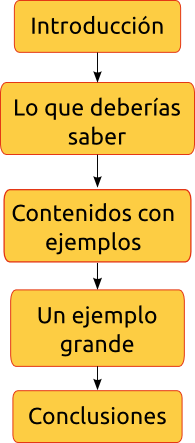
\includegraphics[width=2cm]{img/workflow-iberogre.png} 
    \caption{Flujo de lectura en \wiki}
    \label{img:workflow-iberogre}
\end{figure}

\paragraph{}
A continuación a adjunta una lista de los principales artículos publicados
en \wiki hasta la fecha:

\subsubsection{Artículos publicados}

\begin{itemize}
    \item \textbf{Primeros pasos}
    \begin{itemize}
        \item Comenzando en IberOgre: qué es IberOgre, su filosofía,
        estructura y objetivos.
    \end{itemize}
    \item \textbf{Programación de videojuegos en 3D}: por el momento no
    se ha redactado ningún artículo sobre conocimientos generales de desarrollo
    de videojuegos en 3D.
    \item \textbf{Ogre3D}
    \begin{itemize}
        \item Conociendo Ogre3D: qué es Ogre, sus capacidades y limitaciones.
        Repaso sobre sus características principales.
        \item Conceptos generales: arquitectura y descripción de cada 
        subsistema que compone el motor.
        \item Instalación de Ogre3D 1.7 en GNU/Linux.
        \item Instalación de Ogre3D 1.7 en Windows.
        \item Creación de un entorno de trabajo multiplataforma: explicación
        para establecer un entorno de trabajo (jerarquía de directorios,
        compilación...) para trabajar con proyectos que usen Ogre tanto
        en Windows como en GNU/Linux.
        \item Inicialización y cierre de Ogre: detalles sobre el proceso de
        inicialización, configuración y cierre de Ogre. El primer artículo
        en el que comenzamos a crear aplicaciones.
        \item Gestión de recursos: conocer la forma en la que Ogre gestiona
        recursos como modelos, texturas y esqueletos. Aprender a controlar
        el ciclo de vida de los recursos.
        \item Creación básica de escenas: ventanas, cámaras y carga de modelos
        para construir escenas sencillas.
        \item Manipulación de nodos: gestión de los nodos de la escena, uso
        de transformaciones (movimiento, escala y rotación).
        \item Luces, sombras y entorno: trabajar con efectos de iluminación,
        sombras, efectos de niebla y fondos.
    \end{itemize}
    \item \textbf{Otras tecnologías}
    \begin{itemize}
        \item Manejo básico de OIS: conocimientos sobre la biblioteca de
        gestión de eventos de entrada que se utiliza a lo largo de la wiki.
        \item Exportar modelos desde Blender: proceso de instalación, configuración
        y uso del plugin para exportar modelos desde Blender a Ogre. Consejos
        para conseguir exportaciones óptimas.
        \item Colisiones y físicas con OgreBullet: instalación y uso de
        esta biblioteca de simulación física con cuerpos rígidos para Ogre.
    \end{itemize}
\end{itemize}

\begin{figure}[H]
    \centering
        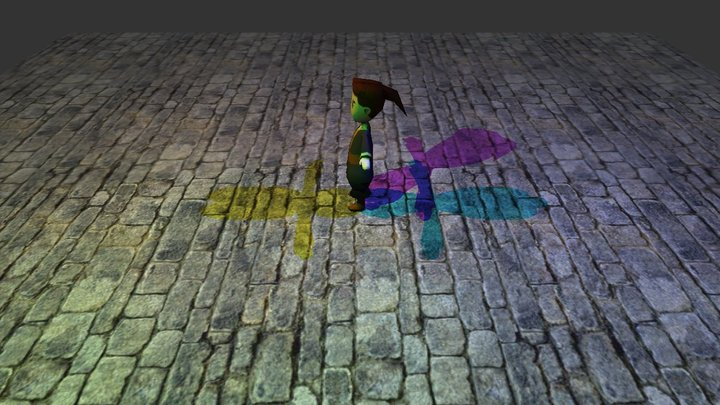
\includegraphics[width=10cm]{img/ejemplo-iberogre.jpg} 
    \caption{Imagen de uno de los ejemplos de 'Luces, sombras y entorno'}
    \label{img:ejemplo-iberogre}
\end{figure}

\begin{figure}[H]
    \centering
        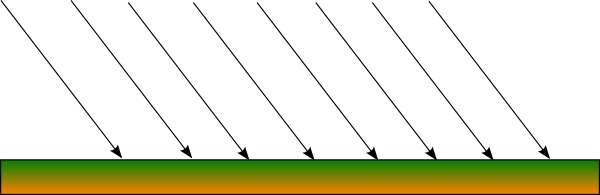
\includegraphics[width=10cm]{img/luz-direccional.png} 
    \caption{Diagrama explicativo de la luz direccional en Ogre}
    \label{img:luz-direccional}
\end{figure}

\subsection{Sion Tower}

\subsubsection{Documento de diseño}

\paragraph{}
Uno de los primeros pasos en el desarrollo de \juego fue la elaboración
de un documento de diseño. Este escrito recoge una descripción del juego,
mecánicas de juego, menús, controles, personajes, enemigos y habilidades.
Finaliza con una lista de recursos artísticos necesarios para el proyecto.
Puede descargarse desde:

\begin{verbatim}
    http://forja.rediris.es/frs/download.php/2019/gdd.pdf
\end{verbatim}

\paragraph{}
Esto me ha permitido conseguir colaboraciones de gran importancia. Los
interesados en el proyecto pueden informarse sobre el mismo, además,
pueden conocer cuáles son las tareas pendientes acudiendo a la lista de
recursos. Todos los artistas han compartido la misma idea de \juego en
términos de estilo gracias a las descripciones.

\subsubsection{Música y efectos de sonido 3D}

\paragraph{}
Ogre no incorpora reproducción de música ni efectos de sonido por lo que fue
necesario desarrollar un sistema propio. Cuenta con las siguientes
funcionalidades:

\begin{enumerate}
    \item Reproducción de música en formato OGG.
    \item Reproducción de efectos de sonido.
    \item Integración total con el sistema de gestión de recursos de Ogre.
    \item Independiente del resto del motor.
    \item Audio 3D: inserción de efectos en nodos de forma que el volumen
    de cada altavoz varía en función de la distancia y el ángulo con respecto
    a la fuente.
\end{enumerate}

\begin{figure}[H]
    \centering
        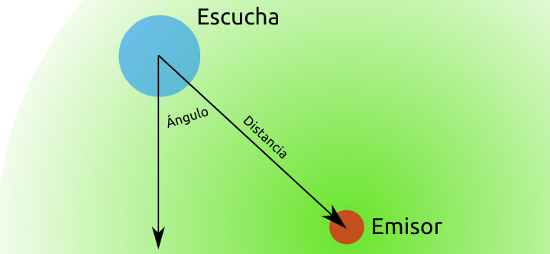
\includegraphics[width=8cm]{img/audio3d.png} 
    \caption{Esquema ilustrando el concepto del audio 3D}
    \label{img:audio3D}
\end{figure}

\paragraph{}
El código fuente está disponible junto a su documentación en:

\begin{verbatim}
http://forja.rediris.es/frs/download.php/2075/siontower-3dsound-v0.1.tar.gz
\end{verbatim}

\subsubsection{Detección de colisiones}

\paragraph{}
Ogre tampoco incorpora detección de colisiones por lo que se ha implementado
un sistema con las características que siguen:

\begin{enumerate}
    \item Basado en formas: esferas, cajas (AABB y OBB) y planos.
    \item Cuerpos colisionables compuestos por varias formas básicas.
    \item Encapsulación de la parte física y visual de los elementos de juego.
    \item Filtrado, detección y respuesta de colisiones mediante callbacks.
\end{enumerate}

\begin{figure}[H]
    \centering
        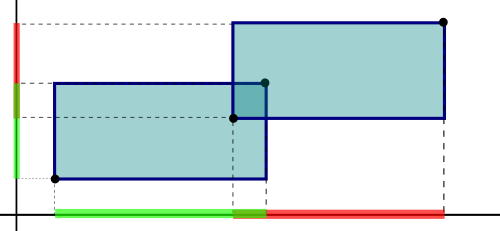
\includegraphics[width=8cm]{img/test-aabb-aabb.png} 
    \caption{Test de colisión entre dos AABBs}
    \label{img:aabb-aabb}
\end{figure}

\paragraph{}
El código fuente está disponible junto a su documentación en:

\begin{verbatim}
http://forja.rediris.es/frs/download.php/2091/siontower-collisions-v0.2.tar.gz
\end{verbatim}

\paragraph{}
En el blog del proyecto se ha publicado una serie compuesta por cinco artículos
documentando a fondo las generalidades y detalles del sistema de detección
de colisiones.

\subsubsection{Carga de escenarios en formato DotScene}

\paragraph{}
El motor de \juego está orientado a la creación de contenidos. Es posible
que los diseñadores o usuarios creen sus propios niveles en Blender. Colocan
objetos del escenario, definen las zonas transitables por los enemigos y
especifican información adicional. Los niveles se exportan a un fichero
XML en formato DotScene que es cargado por el motor. Cuando \juego avance
en su desarrollo se proporcionará un manual al respecto.

\begin{figure}[H]
    \centering
        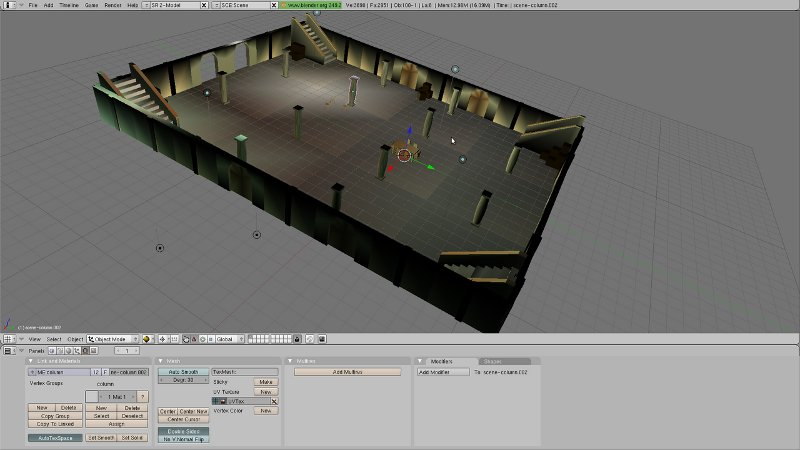
\includegraphics[width=10cm]{img/niveles-blender.jpg} 
    \caption{Creación de niveles desde Blender}
    \label{img:blender}
\end{figure}

\subsubsection{Demo técnica}

\paragraph{}
Con motivo de la fase local del V Concurso Universitario de Software Libre
se publicó una demo técnica de \juego. En la demo se muestra al prototipo
del protagonista moviéndose por el escenario con la detección de colisiones
activada y la música compuesta por los colaboradores. Puede descargarse
a través de los siguientes enlaces:

\begin{verbatim}
http://forja.rediris.es/frs/download.php/2151/siontower-0.1-demo-src.tar.gz
http://forja.rediris.es/frs/download.php/2152/siontower-0.1-demo-win.zip
\end{verbatim}

\begin{figure}[H]
    \centering
        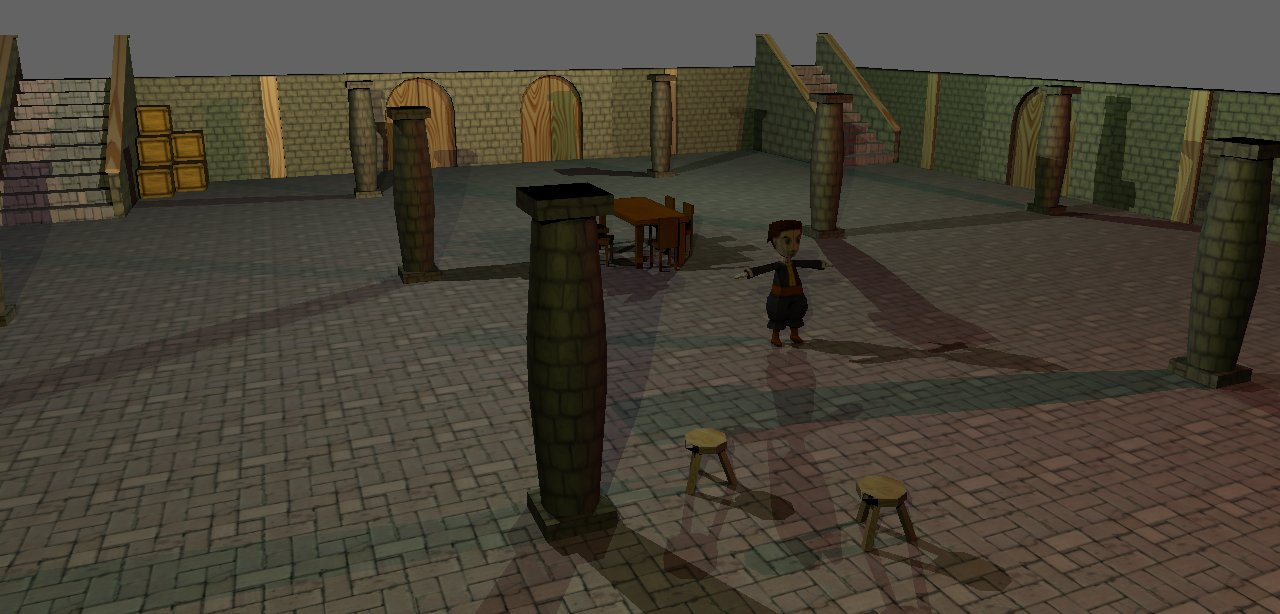
\includegraphics[width=10cm]{img/demo-tecnica.jpg} 
    \caption{Sion Tower 0.1 demo técnica}
    \label{img:demo}
\end{figure}

\paragraph{}
La versión actual de \juego incorpora más características como la búsqueda
de caminos que solo se han mostrado en vídeos en el blog. 

\section{Colaboraciones y difusión}

\paragraph{}
Uno de los mayores logros de \proyecto está siendo el apoyo que recibe de
la comunidad. El apoyo se manifiesta de varias formas: desde sugerencias
o informes de errores hasta artículos nuevos, difusión, colaboraciones
artísticas, etc. A continuación se proporciona una lista de las más relevantes.

\subsection{Aportaciones a IberOgre}

\begin{itemize}
    \item \textbf{Artículo \emph{Conceptos generales}}: Alberto Cejas Sánchez,
    compañero que también participa en el V CUSL con \emph{Fútbol es Así}
    redactó este texto en su totalidad.
    \item \textbf{Artículo \emph{Colisiones con OgreBullet}}: el compañero
    Alberto Cejas Sánchez también ha creado al completo un artículo sobre
    la detección de colisiones con la biblioteca open source OgreBullet.
    \item \textbf{Edición en Wikimedia}: Noelia Sales Montes y Emilio José
    Rodríguez Posada confecionaron una guía liberada bajo Creative Commons
    3.0 by-sa con los conocimientos básicos de edición de artículos en
    sistemas Wikimedia. Es accesible desde la portada de \wiki lo que
    ayudará a conseguir colaboradores adicionales.
    \item \textbf{Traducción del manual oficial}: Mario Velázquez Muñoz,
    alumno de la Universidad Carlos III de Madrid, aportó una traducción
    completa del manual de referencia oficial de Ogre. La traducción formaba
    parte de la documentación de su Proyecto Fin de Carrera y está disponible
    en la portada de \wiki bajo Creative Commons 3.0 by-nc-sa.
    \item \textbf{Otras aportaciones}: otros compañeros como Jesús
    González Rodríguez (\emph{Balloon Breakers}) han aportado artículos nuevos
    y ediciones de los ya existentes.
\end{itemize}

\begin{figure}[H]
    \centering
        
\includegraphics[width=5cm]{img/avatar.jpg} 
    \caption{Protagonista de Balloon Breakers, colaborador de IberOgre}
    \label{img:balloon}
\end{figure}

\subsection{Difusión del proyecto}

\begin{itemize}
    \item \textbf{Comunidades de desarrollo}: varias comunidades de desarollo
    de videojuegos en español han publicado artículos hablando de \proyecto.
    \begin{verbatim}
    http://www.creagames.es/iberogre-un-proyecto-espanol-de-ogre-engine
    http://razonartificial.com/2011/03/iberogre-documentacion-de-ogre-en-espanol
    http://programandoideas.com/2011/01/iberogre-tutoriales-de-ogre3d-en-espanol
    \end{verbatim}
    \item \textbf{Web oficial de Ogre}: \wiki apareció en la portada de
    la web oficial de Ogre dentro de la cuarta sección de noticias.
    \begin{verbatim}
    http://www.ogre3d.org/2011/03/01/ogre-news-4
    \end{verbatim}
    \item \textbf{Twitter}: 65 seguidores de los que se han recibido muchas
    sugerencias y opiniones. Steve Streeting, fundador de Ogre, recomendó
    \wiki a través de este medio.
    \item \textbf{Blog}: más de 60 artículos con 46.000 visitas en el
    periodo del concurso.
\end{itemize}

\begin{figure}[H]
    \centering
        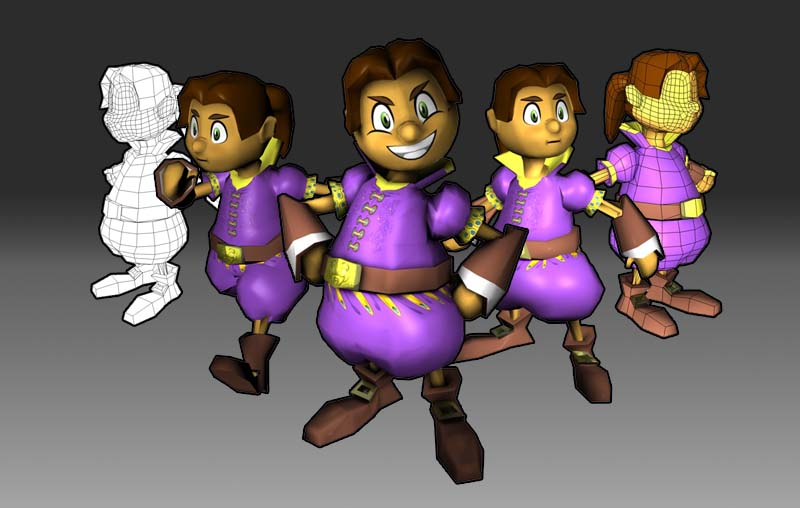
\includegraphics[width=10cm]{img/collage-protagonista.jpg} 
    \caption{Protagonista de \juego por AJR}
    \label{img:protagonista}
\end{figure}


\subsection{Colaboraciones en Sion Tower}

\begin{itemize}
    \item \textbf{Banda sonora original}: el Estudio Evergreen formado por
    Antonio Caro Oca y Daniel Pellicer García están trabajando en una banda
    sonora especialmente compuesta para \juego. Actualmente han terminado
    varias piezas que pueden escucharse en el blog o:
    \begin{verbatim}
    http://estudioevergreen.wordpress.com/canciones
    \end{verbatim}
    \item \textbf{Arte 3D}: AJR (Antonio Jiménez Rodríguez) es diseñador
    gráfico de forma profesional y está trabajando en el arte 3D de los
    personajes (diseño, modelado, texturizado y animación). Su trabajo está
    en el blog de desarrollo y en su blog personal:
    \begin{verbatim}
    http://ajr-portafolio.blogspot.com/
    \end{verbatim}
    \item \textbf{Suavizado de movimientos}: Javier Santacruz López-Cepero
    ha colaborado con un parche para \juego que suaviza las rutas en la
    búsqueda de caminos con la malla de navegación.
\end{itemize}

\begin{figure}[H]
    \centering
        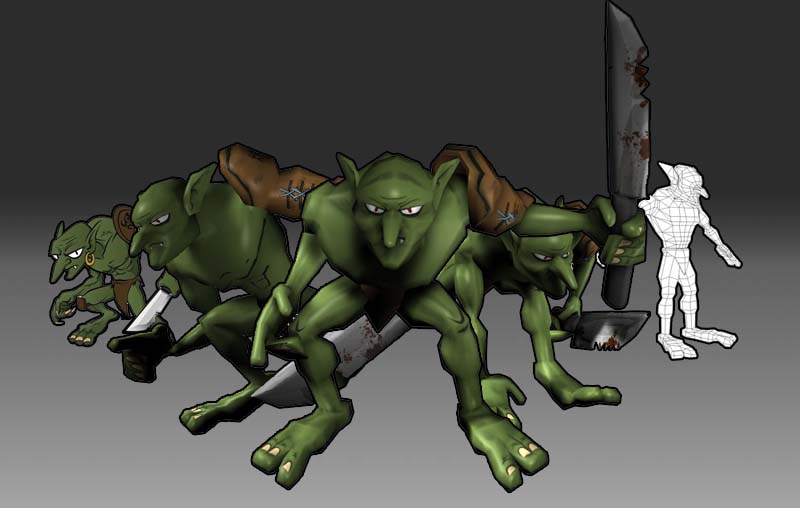
\includegraphics[width=10cm]{img/collage-goblin.jpg} 
    \caption{Enemigo Goblin de \juego por AJR}
    \label{img:protagonista}
\end{figure}


\end{document}
